\documentclass[11pt,a4paper]{article}

%----------------------------- Packages -------------------------------
\usepackage[T1]{fontenc}
\usepackage[utf8]{inputenc}
\usepackage[margin=2.5cm]{geometry}
\usepackage{graphicx}
\usepackage{float}
\usepackage{caption}
\usepackage{booktabs}
\usepackage{xcolor}
\usepackage{listings}
\usepackage[linesnumbered,ruled,vlined]{algorithm2e}
\SetAlgoCaptionSeparator{.}
\usepackage{enumitem}
\usepackage{fancyhdr}
\usepackage{xurl}
\usepackage{tabularx}
\usepackage[hidelinks]{hyperref}
\usepackage{tikz}
\usetikzlibrary{shapes.geometric,arrows.meta,positioning,calc}

%--------------------------- Caption Styling ---------------------------
\captionsetup{labelsep=period}

%--------------------------- Color Definitions ------------------------
\definecolor{codeback}{rgb}{0.97,0.97,0.98}
\definecolor{codegreen}{rgb}{0.15,0.55,0.25}
\definecolor{codegray}{rgb}{0.45,0.45,0.45}
\definecolor{codepurple}{rgb}{0.55,0.15,0.65}
\definecolor{arduinoblue}{rgb}{0.0,0.35,0.65}
\definecolor{sensorgreen}{rgb}{0.15,0.6,0.2}

%--------------------------- Header/Footer ----------------------------
\pagestyle{fancy}
\fancyhf{}
\setlength{\headheight}{14pt}
\lhead{Ultrasonic Distance Measurement System}
\rhead{Abha Singh Sardar}
\cfoot{\thepage}
\renewcommand{\headrulewidth}{0.4pt}

%--------------------------- Code Listing Style ------------------------
\lstdefinestyle{report}{
    backgroundcolor=\color{codeback},
    commentstyle=\color{codegreen}\itshape,
    keywordstyle=\color{blue}\bfseries,
    numberstyle=\tiny\color{codegray},
    stringstyle=\color{codepurple},
    basicstyle=\ttfamily\footnotesize,
    breakatwhitespace=false,
    breaklines=true,
    captionpos=b,
    keepspaces=true,
    numbers=left,
    numbersep=8pt,
    showspaces=false,
    showstringspaces=false,
    showtabs=false,
    tabsize=2,
    frame=single,
    rulecolor=\color{codegray}
}
\lstset{style=report}
\lstset{language=C++}

%=======================================================================
\begin{document}

%------------------------------ Title ---------------------------------
\begin{titlepage}
\pagenumbering{gobble}
\centering
\vspace*{3cm}
{\Huge\bfseries Ultrasonic Distance Measurement System \par}
\vspace{2cm}
{\large
\begin{tabular}{rl}
\textbf{Name}      & Abha Singh Sardar  \\[6pt]
\textbf{SR Number} & 27086             \\[6pt]
\textbf{Module}    & Ultrasonic Sensor Module \\[6pt]
\end{tabular}\par}
\vspace{2.5cm}
{\large \today \par}
\vfill
\end{titlepage}

\newpage
\pagenumbering{arabic}

%--------------------------- Section 1 ---------------------------------
\section{Introduction}

\subsection{Aim}
The aim of this assignment is to design, program, and interface an HC-SR04 ultrasonic sensor with an Arduino Mega 2560 microcontroller to measure obstacle distance continuously and output the values through serial communication.

\subsection{Overview of Approach}
The system utilizes time of flight principles using high-frequency acoustic waves. The microcontroller sends a ten-microsecond high pulse to the trigger terminal of the HC-SR04 sensor. In response, the sensor module transmits an eight-cycle sonic burst at forty kilohertz and drives its echo pin to a high logic state.

By measuring the duration of this echo pulse using the timing functions of the microcontroller, the system computes the physical distance to the reflecting target based on the speed of sound in air. The calculated distance values are continuously output to the serial monitor at a standard communication speed of 9600 baud.

%--------------------------- Section 2 ---------------------------------
\section{Hardware Used}
The experimental apparatus comprises an Arduino Mega 2560 microcontroller board, an HC-SR04 ultrasonic rangefinder module, flexible interconnection cables, and a host workstation.

\subsection{Components}
Table~\ref{tab_components} lists all physical hardware units used in the distance measurement configuration along with their specific technical functions.

\begin{table}[H]
\centering
\begin{tabularx}{\textwidth}{@{}llcX@{}}
\toprule
\textbf{Component} & \textbf{Model / Part} & \textbf{Qty} & \textbf{Purpose} \\
\midrule
Microcontroller Board & Arduino Mega 2560 & 1 & Processing and sensor timing control \\
Ultrasonic Sensor & HC-SR04 & 1 & Distance sensing via time of flight \\
Jumper Wires & Male-to-Female & 4 & Circuit interconnections \\
Host Computer & Personal Computer & 1 & Provides power over USB and visualizes serial telemetry \\
\bottomrule
\end{tabularx}
\caption{Components used in the ultrasonic distance sensing build.}
\label{tab_components}
\end{table}

\subsection{Wiring Diagram}
Figure~\ref{fig_wiring} shows the electrical connections between the Arduino Mega 2560 microcontroller and the HC-SR04 sensor module.

\begin{figure}[H]
\centering
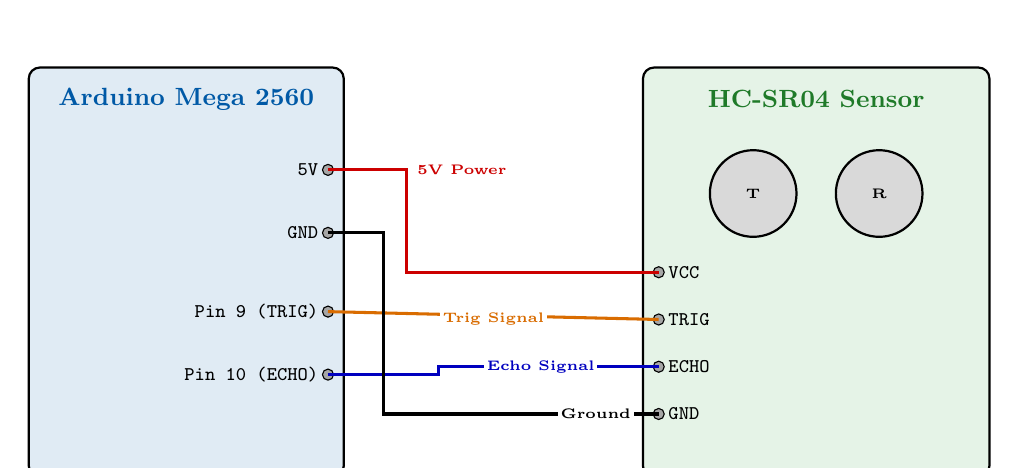
\begin{tikzpicture}[
    box/.style={draw=black, thick, rounded corners=4pt, fill=white, inner sep=5pt},
    pinlabel/.style={font=\ttfamily\scriptsize, text=black},
    wire/.style={line width=1.1pt}
]
    % Arduino Mega 2560
    \node[box, fill=arduinoblue!12, minimum width=4.0cm, minimum height=5.2cm] (mega) at (0, 0) {};
    \node[font=\bfseries\small, text=arduinoblue] at (0, 2.2) {Arduino Mega 2560};

    \node[pinlabel, anchor=east] (m_5v) at (1.8, 1.3) {5V};
    \node[pinlabel, anchor=east] (m_gnd) at (1.8, 0.5) {GND};
    \node[pinlabel, anchor=east] (m_p9) at (1.8, -0.5) {Pin 9 (TRIG)};
    \node[pinlabel, anchor=east] (m_p10) at (1.8, -1.3) {Pin 10 (ECHO)};

    \foreach \p in {m_5v, m_gnd, m_p9, m_p10} {
        \filldraw[fill=gray!70, draw=black] (\p.east) circle (2pt);
    }

    % HC-SR04 Sensor
    \node[box, fill=sensorgreen!12, minimum width=4.4cm, minimum height=5.2cm] (sr04) at (8, 0) {};
    \node[font=\bfseries\small, text=sensorgreen!80!black] at (8, 2.2) {HC-SR04 Sensor};

    % Transducer circles
    \draw[fill=gray!30, draw=black, thick] (7.2, 1.0) circle (0.55cm);
    \node[font=\tiny\bfseries] at (7.2, 1.0) {T};
    \draw[fill=gray!30, draw=black, thick] (8.8, 1.0) circle (0.55cm);
    \node[font=\tiny\bfseries] at (8.8, 1.0) {R};

    % Pins on HC-SR04
    \node[pinlabel, anchor=west] (s_vcc) at (6.0, 0.0) {VCC};
    \node[pinlabel, anchor=west] (s_trig) at (6.0, -0.6) {TRIG};
    \node[pinlabel, anchor=west] (s_echo) at (6.0, -1.2) {ECHO};
    \node[pinlabel, anchor=west] (s_gnd) at (6.0, -1.8) {GND};

    \foreach \p in {s_vcc, s_trig, s_echo, s_gnd} {
        \filldraw[fill=gray!70, draw=black] (\p.west) circle (2pt);
    }

    % Wires with orthogonal routes
    \draw[wire, color=red!80!black] (m_5v.east) -- ++(1.0, 0) |- (s_vcc.west);
    \draw[wire, color=orange!85!black] (m_p9.east) -- (s_trig.west);
    \draw[wire, color=blue!75!black] (m_p10.east) -- ++(1.4, 0) |- (s_echo.west);
    \draw[wire, color=black] (m_gnd.east) -- ++(0.7, 0) |- (s_gnd.west);

    % Wire labels
    \node[font=\tiny\bfseries, text=red!80!black, fill=white, inner sep=1pt] at (3.5, 1.3) {5V Power};
    \node[font=\tiny\bfseries, text=orange!85!black, fill=white, inner sep=1pt] at (3.9, -0.6) {Trig Signal};
    \node[font=\tiny\bfseries, text=blue!75!black, fill=white, inner sep=1pt] at (4.5, -1.2) {Echo Signal};
    \node[font=\tiny\bfseries, text=black, fill=white, inner sep=1pt] at (5.2, -1.8) {Ground};

\end{tikzpicture}
\caption{Circuit diagram for interfacing Arduino Mega 2560 with HC-SR04 sensor.}
\label{fig_wiring}
\end{figure}

The VCC terminal of the HC-SR04 module connects to the regulated five-volt terminal of the Arduino Mega 2560 board, and GND connects to common system ground. Digital pin 9 supplies the initiating trigger pulse, while digital pin 10 reads the duration of the returning echo pulse.

%--------------------------- Section 3 ---------------------------------
\section{Logic Used and System Flowchart}
The measurement logic relies on precise pulse timing to determine the round-trip acoustic transit delay. Sound travels through dry air at approximately three hundred forty-three meters per second at standard room temperature, corresponding to zero point zero three four three centimeters per microsecond.

A measurement cycle begins by asserting a low state on the trigger line for two microseconds to establish a clear baseline. Next, the microcontroller raises the trigger pin high for ten microseconds before restoring it to low. This pulse commands the internal electronics of the HC-SR04 to transmit an eight-cycle sonic wave packet at forty kilohertz.

Following transmission, the sensor brings the echo pin high. The echo pin remains high while the sound waves travel to the obstacle and reflect back to the receiver transducer. The pulseIn timing routine records the high-level duration in microseconds. Because the sound waves complete a round trip, dividing the product of elapsed duration and sound velocity by two yields the one-way distance to the target.

\subsection{System Flowchart}
Figure~\ref{fig_flowchart} illustrates the sequential runtime execution loop for ultrasonic distance measurement.

\begin{figure}[H]
\centering
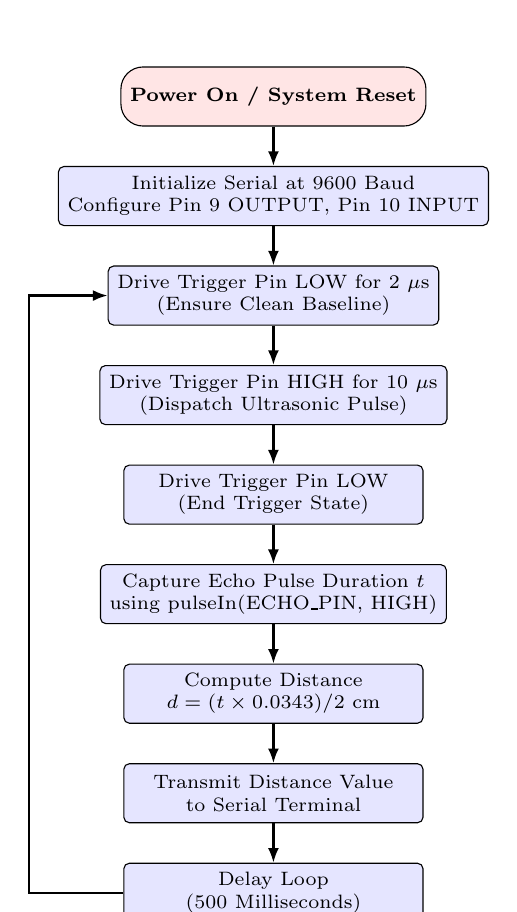
\begin{tikzpicture}[
    node distance=0.8cm,
    startstop/.style={rectangle, rounded corners=8pt, minimum width=3.8cm, minimum height=0.75cm, text centered, draw=black, fill=red!10, font=\scriptsize\bfseries},
    process/.style={rectangle, rounded corners=2pt, minimum width=3.8cm, minimum height=0.75cm, text centered, draw=black, fill=blue!10, font=\scriptsize, align=center},
    arrow/.style={thick, -{Latex[scale=0.8]}}
]
    \node[startstop] (start) {Power On / System Reset};
    \node[process, below=0.5cm of start] (init) {Initialize Serial at 9600 Baud\\Configure Pin 9 OUTPUT, Pin 10 INPUT};
    \node[process, below=0.5cm of init] (trig_low1) {Drive Trigger Pin LOW for 2 $\mu$s\\(Ensure Clean Baseline)};
    \node[process, below=0.5cm of trig_low1] (trig_high) {Drive Trigger Pin HIGH for 10 $\mu$s\\(Dispatch Ultrasonic Pulse)};
    \node[process, below=0.5cm of trig_high] (trig_low2) {Drive Trigger Pin LOW\\(End Trigger State)};
    \node[process, below=0.5cm of trig_low2] (measure) {Capture Echo Pulse Duration $t$\\using pulseIn(ECHO\_PIN, HIGH)};
    \node[process, below=0.5cm of measure] (calc) {Compute Distance\\$d = (t \times 0.0343) / 2$ cm};
    \node[process, below=0.5cm of calc] (serial) {Transmit Distance Value\\to Serial Terminal};
    \node[process, below=0.5cm of serial] (delay) {Delay Loop\\(500 Milliseconds)};

    \draw[arrow] (start) -- (init);
    \draw[arrow] (init) -- (trig_low1);
    \draw[arrow] (trig_low1) -- (trig_high);
    \draw[arrow] (trig_high) -- (trig_low2);
    \draw[arrow] (trig_low2) -- (measure);
    \draw[arrow] (measure) -- (calc);
    \draw[arrow] (calc) -- (serial);
    \draw[arrow] (serial) -- (delay);
    \draw[arrow] (delay.west) -- ++(-1.2,0) |- (trig_low1.west);

\end{tikzpicture}
\caption{Flow diagram of the ultrasonic distance measurement process.}
\label{fig_flowchart}
\end{figure}

\subsection{Algorithmic Structure or Pseudocode}
Algorithm~\ref{algo_ultrasonic} details the sequential execution implemented in the microcontroller firmware.

\begin{algorithm}[H]
\DontPrintSemicolon
\caption{Distance measurement using ultrasonic sensor}
\label{algo_ultrasonic}
Initialize serial communication at 9600 baud rate \\
Configure digital pin 9 as output for trigger \\
Configure digital pin 10 as input for echo \\
Drive trigger pin 9 to low state \\
\BlankLine
\While{true}{
    Set trigger pin to low for two microseconds to clear line \\
    Set trigger pin to high for ten microseconds to send pulse \\
    Set trigger pin to low \\
    \BlankLine
    Record echo pin high duration in microseconds as t \\
    Calculate distance d as t multiplied by 0.0343 divided by 2 \\
    \BlankLine
    Output distance d to serial monitor \\
    Wait for five hundred milliseconds \\
}
\end{algorithm}

%--------------------------- Section 4 ---------------------------------
\section{Code}
The complete Arduino C++ program compiled and loaded onto the microcontroller board is presented below.

\begin{lstlisting}
// HC-SR04 Ultrasonic Distance Measurement
// Arduino Uno / ATmega328P

const int trigPin = 9;
const int echoPin = 10;

long duration;
float distance;

void setup() {
  Serial.begin(9600);

  pinMode(trigPin, OUTPUT);
  pinMode(echoPin, INPUT);

  digitalWrite(trigPin, LOW);
}

void loop() {

  // Send a 10 microsecond ultrasonic pulse
  digitalWrite(trigPin, LOW);
  delayMicroseconds(2);

  digitalWrite(trigPin, HIGH);
  delayMicroseconds(10);
  digitalWrite(trigPin, LOW);

  // Measure the time taken by the echo
  duration = pulseIn(echoPin, HIGH);

  // Calculate distance
  // Speed of sound = 343 m/s
  // Distance (cm) = duration * 0.0343 / 2
  distance = duration * 0.0343 / 2;

  // Display distance
  Serial.print("Distance: ");
  Serial.print(distance);
  Serial.println(" cm");

  delay(500);
}
\end{lstlisting}

\newpage
%--------------------------- Section 5 ---------------------------------
\section{Results}
The ultrasonic rangefinder interface was validated by positioning reflective obstacles at varying separations from the sensor assembly. The microcontroller transmitted periodic ten-microsecond trigger excitation pulses and recorded the returning acoustic echo transit duration.

Figure~\ref{fig_results_ultra} illustrates the real-time distance measurements streamed to the serial terminal at 9600 baud rate. The system consistently calculated obstacle distances across multiple ranges, demonstrating reliable performance around thirty-five to forty-two centimeters during proximate object tracking as well as extended distances up to two hundred eighty-four centimeters. Periodic high readings correspond to clear sightlines where reflected acoustic pulses exceeded the measurement timeout threshold. The experimental findings confirm linear acoustic transit timing and stable range determination across the measurement envelope.

\begin{figure}[H]
\centering
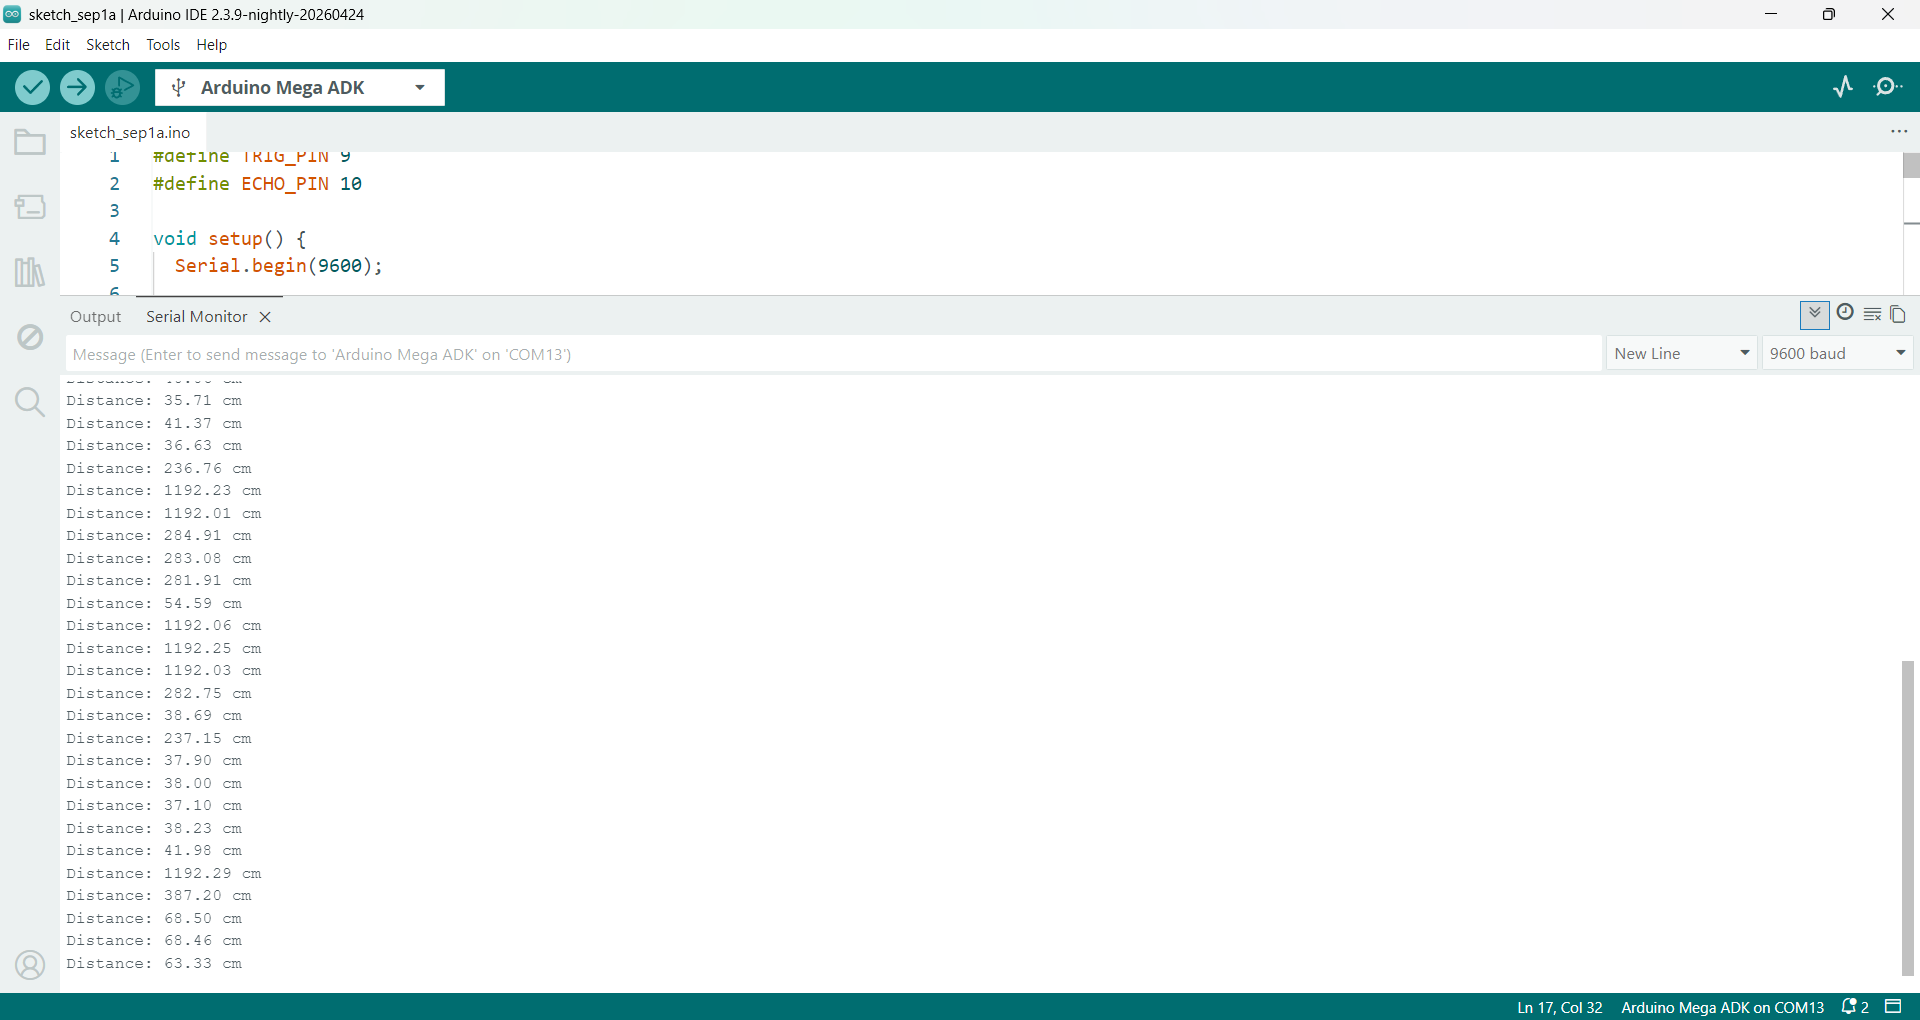
\includegraphics[width=0.72\linewidth]{Ultra.png}
\caption{Serial monitor output captured during ultrasonic distance measurements.}
\label{fig_results_ultra}
\end{figure}

%--------------------------- Section 6 ---------------------------------
\section{Video}
The recorded experimental demonstration verifying the operation of the ultrasonic sensor system is accessible on the course SharePoint repository.

\vspace{0.4cm}
\begin{center}
\href{https://indianinstituteofscience.sharepoint.com/:v:/s/MN2072026-27Aug-Dec/IQAXWQUAvupDQKJuZv8jrF8iAfm_GRK9Yv9i-EPQQV_qD8Y?e=ImhmVb}{\large \textbf{Click Here to View the Ultrasonic Sensor Demonstration Video}}
\end{center}

\vspace{0.4cm}
\noindent
The complete web link for manual browser access is provided below.

\vspace{0.2cm}
\noindent
{\footnotesize \url{https://indianinstituteofscience.sharepoint.com/:v:/s/MN2072026-27Aug-Dec/IQAXWQUAvupDQKJuZv8jrF8iAfm_GRK9Yv9i-EPQQV_qD8Y?e=ImhmVb}}

\end{document}
